Las perovskitas son materiales que combinan elementos met\'alicos y no met\'alicos en una estructura de tipo fcc. Esta estructura cristalina contiene dos cationes met\'alicos siendo uno m\'as peque\~no que el otro, y un anion no met\'alico. A esta estructura se le suele representar como $ABO_{3}$ y posee una celda c\'ubica donde se ubica al cati\'on {\bf A} en el centro, al cati\'on {\bf B} en los v\'ertices y al ani\'on {\bf O} en los puntos medios de los espacios que separan a los cationes {\bf B}. Esta representaci\'on es la octa\'edrica (figura \ref{perovskita_cubica}) y a los materiales que presentan esta estructura se les llama perovskitas ideales \cite{inigues2008}.

\noindent Las perovskitas ideales se comportan como aislantes y presentan isotrop\'ia en sus propiedades el\'ectricas, \'opticas y mec\'anicas debido a que los ejes de su estructura cubica son id\'enticos. Pero en la realidad las perovskitas presentan distorsiones debido a que un cati\'on met\'alico es m\'as grande que el otro, esto causa un desplazamiento de los aniones y del los cationes m\'as peque\~nos provocando que la estructura cristalina cambie de c\'ubica a ligeramente tetragonal creando momentos dipolares \cite{nicola2000}.

% ------------------------
% poner figura aqui
%----------------------------
\begin{figure}[H]
    \centering
    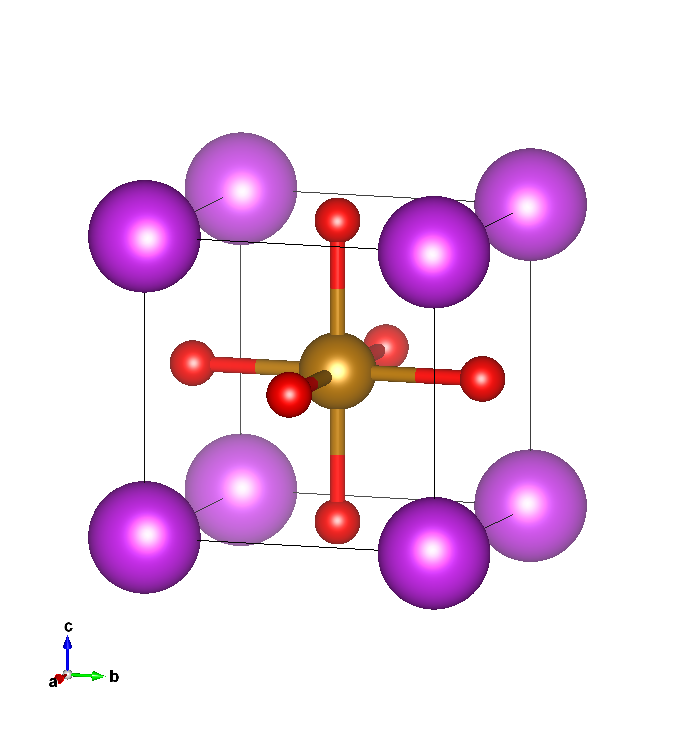
\includegraphics[width=0.4\textwidth]{contenido/marco_teorico/perovskitas/img_Perovskitas/perovskita_cubica.png}
    \caption{Estructura de la perovskita ideal.}
    \label{perovskita_cubica}
\end{figure}

\noindent Los distintos elementos que pueden formar perovskitas son muchos debido a la libertad que existe al escoger los cationes met\'alicos, los cuales pueden ser de elementos diferentes. Por ejemplo, el cati\'on {\bf A} puede ser un metal alcalino, alcalino terreo o tierra rara y el cati\'on {\bf B} habitualmente es un metal de transici\'on, esto da origen a muchas combinaciones con diferentes propiedades \cite{inigues2008}.

\noindent Por ejemplo, el $BaTiO_{3}$ es un diel\'ectrico de alta  susceptibilidad, el$YBaCuO$ es un superconductor de alta temperatura cr\'itica y el $BiFeO_{3}$ tiene un comportamiento multiferr\'oico.


\subsection{Distorciones octa\'edricas}

Como se mencion\'o en la secci\'on anterior, los materiales con estructura de perovskita no poseen una estructura ideal y es m\'as com\'un que posean una estructura tetragonal u ortorr\'ombica. En estos casos los aniones no met\'alicos forman octaedros alrededor del cati\'on met\'alico {\bf B}. Pero estos octaedros no se encuentran alineados con los ejes de la estructura cristalina debido al tama\~no diferente de los cationes met\'alicos \cite{inigues2001}.


\begin{figure}[H]
    \centering
    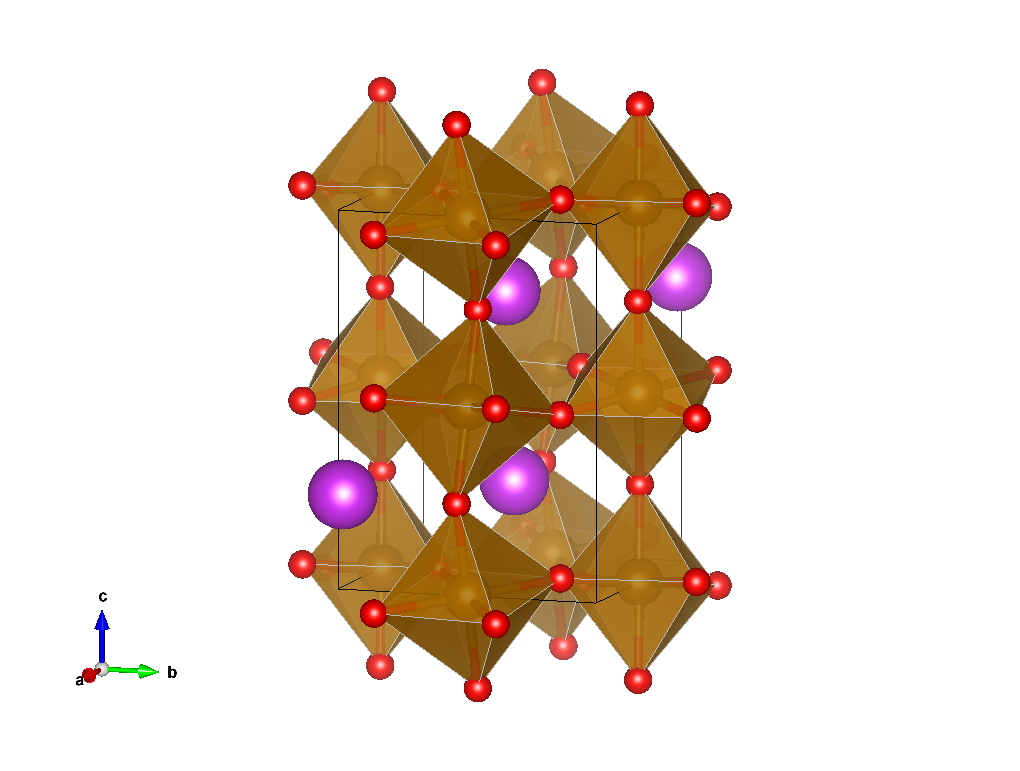
\includegraphics[width=0.6\textwidth]{contenido/marco_teorico/perovskitas/img_Perovskitas/octaedro_perovs.png}
    \caption[Deformaci\'on octaedrica de la perovskita]{Estructura de la 
        perovskita donde se observan 
        deformaciones octa\'edricas.}
    \label{perovskita_octaedro}
\end{figure}

\noindent Las distorsiones octa\'edricas pueden ser clasificadas en dos tipos seg\'un Glazer quien las estudio en el a\~no 1972 creando adem\'as una nomenclatura para denotar las distorsiones. El primer tipo son las distorsiones en fase que presentan octaedros rotados en la misma direcci\'on en torno a un eje y se les asigna el super\'indice (+). El segundo tipo son las distorsiones en antifase que presentan octaedros rotados en sentidos opuestos entre s\'i de forma alternada y se les asigna el super\'indice (-). En caso no exista rotaci\'on de los octaedros se le asigna el super\'indice (0).

\noindent Las fases cristalinas de los materiales estudiados en este trabajo presentan distorsiones octa\'edricas pero un an\'alisis de estas distorsiones octa\'edricas no es parte de los objetivos del trabajo. Sin embargo se mencionan a continuaci\'on algunos de los efectos descritos por Glazer .

\begin{itemize}
    \item {\bf Par\'ametro de red:} La figura (\ref{para_octa}) representa la rotaci\'on octa\'edrica sobre uno de los ejes de la estructura cristalina perpendicular al plano de la imagen. Se observa que los ocatedros consecutivos (negrop - rojo) estan rotados en sentido opuesto, entonces las posiciones se repiten cada dos octaedros (negro - negro) o (rojo - rojo) \cite{glazer1975}.
    \begin{figure}[H]
        \centering
        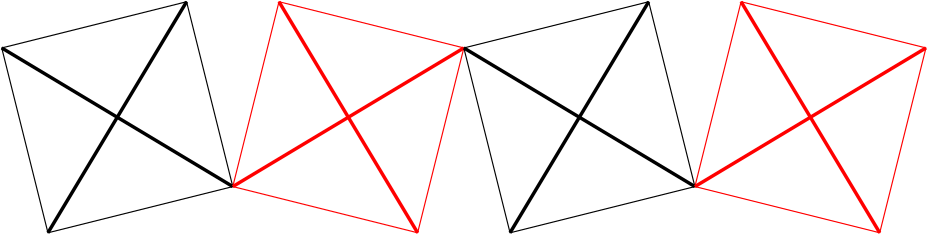
\includegraphics[width=0.6\textwidth]{contenido/marco_teorico/perovskitas/img_Perovskitas/rotacion_octaedrica.png}
        \caption[Rotaci\'on octa\'edrica]{Representaci\'on esquem\'atica de la 
            rotaci\'on octa\'edrica en uno de los ejes de la estructura cristalina.}
        \label{para_octa}
    \end{figure}
    \item {\bf Reflexiones adicionales en el patr\'on de difracci\'on:} Las distorsiones octa\'edricas duplican la distancia de repetici\'on tambi\'en conocidas como distancias interplamares. Lo que da origen a reflexiones adicionales en los patrones de difracci\'on de rayos X \cite{glazer1975}.
\end{itemize} 
